\section{Theorie}
Die Strahlung, die in diesem Versuch untersucht wird, ist die $gamma$-Strahlung. Diese elektromagnetische Strahlung ist höherenergetisch als Röntgenstrahlung mit Energien von mindestens $\SI{100}{keV}$. Sie entsteht bei Übergängen zwischen Anregungszuständen im Atomkern. $\gamma$-Strahlung ist nicht direkt beobachtbar, sie muss also erst mit Materie wechselwirken. Die Produkte dieser Wechselwirkung (im Normalfall Elektronen) sind dann beobachtbar.
\subsection{Wechselwirkung von $\gamma$-Strahlung mit Materie}
In diesem Versuch werden die drei häufigsten Prozesse betrachtet: der Photoeffekt, der Compton-Effekt und die Paarbildung.
\subsubsection{Photoeffekt}
Beim Photoeffekt löst das Photon ein Elektron aus der Atomhülle eines Atoms heraus und wird dabei selbst absorbiert. Ein Teil der Energie des Photon wird dabei für die Austrittsarbeit $W_\text{A}$ verwendet, den Rest erhält das Elektron als kinetische Energie. Dieses Elektron kann nun detektiert werden. Da zur Impulserhaltung während des Vorgangs ein weiteres Teilchen benötigt wird, werden meist Elektronen aus inneren Schalen gelöst, sodass der zusätzliche Impuls an den Atomkern abgegeben werden kann. Den freien Platz in der Atomhülle nimmt nun ein Elektron aus einer höheren Schale ein, dass dabei Röntgenstrahlung oder ein Augerelektron abgibt. In beiden Fällen kann die Energie schlussendlich vom Detektor gemessen werden, sodass die gesamte Energie des ursprünglichen $\gamma$-Quants nachgewiesen werden kann.

\subsubsection{Comptoneffekt}
Beim Comptoneffekt streut das $\gamma$-Photon an einem quasifreien Elektron, also einem Elektron der äußeren Atomhülle. Dabei wird ein Teil der Energie des Photons auf das Elektron übertragen, welches in einem Winkel $\theta$ zur ursprünglichen Bahn des Photons abgelenkt wird. Das Photon wird dabei um den Winkel $-\theta$ gestreut und besitzt die verringerte Energie $E_\gamma'$. Die Energie des Elektrons nach dem Stoß lässt sich mit \cref{eq:compton} berechnen.

\begin{equation}
	E_e = E_\gamma \left( 1-\frac{1}{1 + \frac{E_\gamma}{m_ec^2}\left( 1-\cos\left(\theta\right)\right)}\right)
	\label{eq:compton}
\end{equation}

Die übertragene Energie ist also vom Winkel abhängig. Während bei einem Winkel von $0$° keine Energie übertragen wird, ist die Energie bei einem Winkel von $180$° maximal. Unter welchem Winkel die Teilchen streuen ist dabei statistisch verteilt. Wenn also nur gestreutes Elektron detektiert wird, kann daraus ohne Information über den Winkel keine Information über die ursprüngliche Energie des $\gamma$-Quants gewonnen werden. Wenn aber sehr viele Photonen detektiert werden entsteht ein kontinuierliches Spektrum mit einer deutlichen Kante bei der Energie, die das Elektron bei einem Stoß um $180$° erhalten hat, der Comptonkante. Daraus sind Rückschlüsse auf die Energie des Photons möglich.

\subsubsection{Paarbildung}
Der dritte auftretende Effekt nennt sich Paarbildung. Hierbei erzeugt das Photon ein Elektron-Positron-Paar und annihiliert dabei. Die Energie muss mindestens $\SI{1022}{keV}$ betragen, da diese als Ruhemasse der entstehenden Teilchen benötigt wird. Der Rest geht in kinetische Energie der Teilchen über. Dieser Prozess kann nur in Materie stattfinden, da ein weiterer Reaktionspartner (meistens ein Atomkern) benötigt wird, um den überschüssigen Impuls aufzunehmen. Das Elektron kann in diesem Zustand bereits detektiert werden, das Positron allerdings bildet zuerst mit einem anderen Elektron zusammen Positronium. Dieser Zustand zerfällt allerdings nach einiger Zeit und erzeugt so einige Photonen (die Anzahl ist abhängig von den Spins der beiden Teilchen). Diese können nun wiederum über einen der beschriebenen Effekte Elektronen erzeugen, die detektiert werden können. Die Wahrscheinlichkeit, dass einer der oben genannten Prozesse auftritt, steigt mit zunehmender Ladungszahl des Absorbermaterials. Daher werden für die Detektoren schwere Elemente wie z.B. Blei verwendet. Außerdem ist die Wahrscheinlichkeit abhängig von der Energie des Photons. Dieser Zusammenhang ist in \cref{streuung} dargestellt.

\begin{figure}
	\centering
	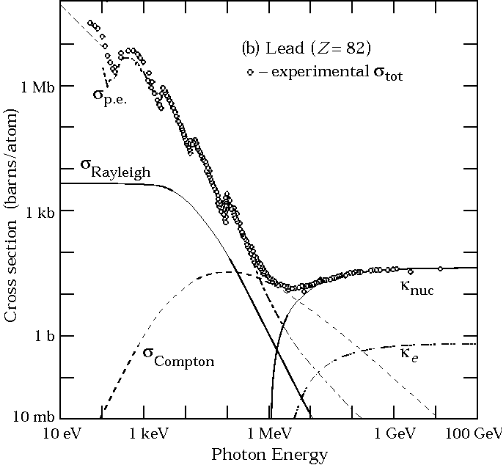
\includegraphics[width=0.9\textwidth]{streuung.png}
	\caption{Dargestellt ist der Wirkungsquerschnitt der einzelnen Effekte in Abhängigkeit von der Energie des Photons in Blei. Bei niedrigen Energien dominiert der Photoeffekt, bei mittleren der Comptoneffekt, bei hohen die Paarbildung. Die Kanten beim Photoeffekt kommen zustande, da genau bei dieser Energie das Photon genug Energie hat, um Elektronen aus einer weiteren, tieferen Schale zu lösen.}
	\label{streuung}
\end{figure}

Bei niedrigen Energien überwiegt der Photoeffekt, bei mittleren Energien zwischen $\SI{300}{keV}$ und $\SI{7}{MeV}$ überwiegt der Comptoneffekt, anschließend die Paarbildung.

\subsection{Detektoren}
In diesem Versuch werden zwei verschiedene Detektorentypen verwendet: Ein Halbleiterdetektor und ein Szintillationsdetektor. der Halbleiterdetektor besteht aus mit Lithium dotiertem Germanium, der Szintillator ist ein Natriumjodid-Kristall, der mit Thallium aktiviert ist. Beide Detektoren wandeln die auftreffende $\gamma$-Strahlung in Elektronen um,  die dann mithilfe verschiedener Bauteile in ein messbares Signal umgewandelt werden können, allerdings auf unterschiedliche Weise. Beide Möglichkeiten werden im folgenden kurz vorgestellt.

\subsubsection{Halbleiterdetektor}
In Halbleitern wird durch auftreffende Photonen ein Elektron-Loch-Paar erzeugt. Dies kann, wenn an den Halbleiter eine Spannung anliegt, abgezogen und gemessen werden. Allerdings wäre hierfür ein hochreiner intrinsischer Halbleiter nötig, da sonst Blindsträme auftreten, die eine gute Messung unmöglich machen. Alternativ wird daher ein sogenannter intrinsic-Kristall verwendet. Bei diesem werden in einen p-dotierten Halbleiter Lithiumatome gegeben, die als n-Dotierung wirken und so die p-Dotierung ausgleichen. Diese Kristalle haben sehr ähnliche Eigenschaften wie intrinsische Halbleiter. So können Sperrschichten mit einer Größe von mehreren Zentimetern zu erzeugen. Die Breite der Sperrschicht ist dabei proportional zur Quadratwurzel der angelegten Spannung. Diese Kristalle werden als pn-Übergang in Sperrrichtung betrieben. Trifft nun ein Photon auf den Kristall, entstehen Elektron-Loch-Paare, die sofort durch die anliegende Spannung getrennt werden und so am rekombinieren gehindert werden. Diese Teilchen erzeugen durch Stöße weitere Elektron-Loch-Paare. Durch die anliegende Hochspannung werden die Ladungsträger aus dem Halbleiter abgezogen und können als Strom gemessen werden.

\subsubsection{Szintillationsdetektor}
Ein Szintillationsdetektor besteht aus zwei Komponenten, dem Szintillator und dem Photomultiplier. Im Szintillator wird die hochenergetische $\gamma$-Strahlung in niederenergetisches sichtbares Licht umgewandelt. Organische Szintillatoren nutzen zur Umwandlung der Strahlung Molekülanregungen, in anorganischen Szintillatoren entstehen das sichtbare Licht durch Übergänge in den Bändern des Kristalls. Durch die auftreffende Strahlung wird ein Elektron-Loch-Paar erzeugt, das anschließend rekombiniert und ein Photon mit der Energie der Bandlücke abgibt. Da dieses Photon an anderen Atomen des Szintillators wieder ein Elektron-Loch-Paar erzeugen und daher den Kristall nicht verlassen würde, werden sogenannte Aktivatoren in den Kristall gegeben. Dies sind Atome mit anderer Bandlücke. Die so entstehenden Photonen erzeugen also mit geringerer Wahrscheinlichkeit wieder ein Elektron-Loch-Paar und können den Kristall verlassen. Anschließend gelangen die Photonen in den Photomultiplier. Dort schlagen die Photonen an einer Kathode Elektronen aus. Diese werden nun durch ein elektrisches Feld auf Dynoden gelenkt, an denen sie nun Sekundärelektronen erzeugen. Diese wiederum erzeugen an der nächsten Dynode weitere Sekundärelektronen, sodass am Ende ein messbares Signal vorliegt.

\subsection{Aufbau}
Um die detektierten Elektronen in ein messbares Signal zu verwandeln, werden noch einige Bauteile benötigt. Zuerst wird das Signal von einem Vorverstärker auf eine Spannung von einigen $100$ mV verstärkt, um es über ein Kabel übertragen zu können. Dabei bekommt es die Form eines exponentiellen Abfalls. Anschließend wird es von einem Hauptverstärker weiter verstärkt und zu einem gaußförmigen Signal geformt, sodass es von den weiteren Bauteilen verarbeitet werden kann. Nun wird das Signal von einem Analog-Digital-Wandler digitalisiert. Zuletzt sortiert ein Multi-Channel-Analyzer die Pulse nach ihrer Energie in verschiedene Kanäle ein. Der hier verwendete MCA besitzt etwa $8000$ verschiedene Channels. Dieser wurde am Anfang mit der Probe, bei der die höchsten Energien zu erwarten waren, so eingestellt, dass alle Channels verwendet werden. So kann die bestmögliche Auflösung sichergestellt werden.

\subsection{$\gamma$-Spektrum}
Die Signale, die auf die verschiedenen Channels des MCA verteilt wurden, können nun am Computer dargestellt werden. Signale, die auf denselben Channel geschickt wurden, werden aufsummiert, sodass die Anzahl der Ereignisse für verschiedene Energien des detektierten Elektrons dargestellt wird. Da die Energie des detektierten Elektrons proportional zur Energie des $\gamma$-Quants ist, können so Rückschlüsse die $\gamma$-Strahlung gezogen werden. Das erwartete Spektrum, idealisiert, ohne Rauschen, ist in \cref{idealized_spectrum} dargestellt.

%\begin{figure}
%	\centering
%	\includegraphics[width=0.9\textwidth]{idealized_spectrum.png}
%	\caption{Idealisiertes Spektrum der $\gamma$-Strahlung. Ganz rechts der Full Energy Peak, der durch den Photoeffekt und bei der Paarbildung, wenn beide durch Zerstrahlung des Positrons entstandenen Photonen noch im Detektor reagieren. Daneben der Single Escape Peak, der auftritt, wenn eines der vom Positron erzeugten Photonen nicht mehr im Detektor reagiert und ganz links der Double Escape Peak, für den Fall, dass beide Photonen nicht reagieren. Zwischen Single Escape Peak und Full Energy Peak ist die Comptonkante zu sehen, die bei Compton-Streuung um $180$° auftritt. Bei niedrigeren Energien ist daneben die kontinuierliche Verteilung für die Streuung unter anderen Winkeln sichtbar}
%	\label{idealized_spectrum}
%\end{figure}

Der Hauptpeak ist der sogenannte Full Energy Peak. Er tritt auf, wenn die gesamte Energie des $\gamma$-Quants im Detektor gemessen wird. Dies ist vor allem der Fall beim Photoeffekt. Er tritt außerdem beim Comptoneffekt auf, wenn sowohl das gestreute Photon als auch das Elektron detektiert werden. Bei der Paarbildung zerstrahlt nach kurzer Zeit das Positronium und erzeugt dabei meist zwei Photonen. Wenn diese beide noch im Detektor durch andere Wechselwirkungen Elektronen erzeugen, die vom Detektor erfasst werden, trägt auch dieser Effekt um Full Energy Peak bei. Wenn jedoch eines der Photonen nicht mehr im Detektor wechselwirkt, trägt dieser Vorgang zum Single Escape Peak bei. Dieser ist zum Full Energy Peak um $\SI{511}{keV}$ zu tieferer Energie verschoben. Entkommen beide Photonen aus dem Detektor entsteht der Double Escape Peak, welcher um $\SI{1022}{keV}$ zum Full Energy Peak verschoben ist. Da beim Comptoneffekt ein kontinuierliches Spektrum an Elektronen, abhängig vom Streuwinkel, entsteht, ist dieser Effekt auch als kontinuierliche Verteilung zwischen den Energien $0$ und $E_\text{max}$ sichtbar. Ab $E_\text{max}$ tritt dieser Effekt nicht mehr auf, daher ist an dieser Stelle die bereits erwähnte Comptonkante zu sehen.

Es auch werden aber auch noch andere Elektronenenergien gemessen, um die das Ergebnis am Ende bereinigt werden muss. Der sogenannte Backscatteruntergrund entsteht durch Compton-Streuung der $\gamma$-Quanten am Abschirmmaterial. Dabei kann ein Photon mit Energien zwischen $E_\text{min}$ und $E_\gamma$ zurück in den Detektor gelangen und dort zum Signal beitragen. So entsteht eine weitere kontinuierliche Verteilung mit Energien zwischen $E_\text{min}$ und $E_\gamma$. Außerdem können durch Photoeffekt am Abschirmmaterial weitere Peaks entstehen, die genau den Energieabständen zwischen zwei Schalen in der Atomhülle dieser Elemente entsprechen.

\section{Auswertung}
\subsection{Kalibration}
Zunächst muss die Kalibrierung bestimmt werden. Dies ist nötig, da die verschiedenen Zählungen in "Channels" unterteilt wurden. Um die Messungen allerdings sinnvoll zu verwenden, ist es nötig die korrespondierenden Energien, zu den jeweiligen Channels zu kennen. Dafür wird zunächst die Messung der $^{22}$Na in \cref{Kali} betrachtet.

\begin{figure}[ht]
	\centering
	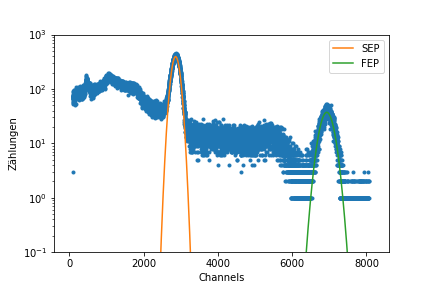
\includegraphics[scale=0.8]{na.png}
	\caption{Messung des $^{22}$Na Spektrums mithilfe des Szintillators.}
	\label{Kali}
\end{figure}

in der Messung sind deutlich zwei Peaks zu sehen, einen Full Energy Peak(FEP) und einen Single Escape Peak(SEP). Da die Literaturwerte der beiden Peaks mit $E_{FEP} = \SI{1274.5}{keV}$ und $E_{SEP} = \SI{511}{keV}$ bekannt sind und außerdem ein linearer Zusammenhang zwischen den Channels und den zugehörigen Energien besteht, kann eine Umrechnung stattfinden.
Das passiert mit der Formel:
\begin{equation}
	E = m \cdot Ch + E_{0},
\end{equation}  
wobei
\begin{equation}
	m = \frac{E_{FEP} - E_{SEP}}{Ch_{FEP} - Ch_{SEP}}
\end{equation}
und 
\begin{equation}
	E_{0} = E_{FEP} - m \cdot Ch_{FEP}
\end{equation}
mit $Ch$ dem jeweilig zugehörigem Channel. Für den Szintillator ergibt das eine Umrechnung von $m = \SI{0,187 \pm 0,007}{\frac{keV}{Ch}}$ und $E_{0} = \SI{-26 \pm 46}{keV}$. Die Umrechnung für den Halbleiter funktioniert analog und ergibt einen Faktor von $m = \SI{0,1699 \pm 0,0004}{\frac{keV}{Ch}}$ und $E_{0} = \SI{0 \pm 3}{keV}$. 

\subsection{$\gamma$-Spektren}
\subsubsection{$^{22}$Na Szintillator}
\begin{figure}[ht]
	\centering
	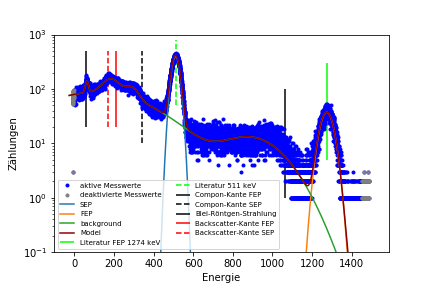
\includegraphics[scale=0.8]{na_sz_.png}
	\caption{$^{22}$Na Szintillator Spektrums auf die korrekten Energien kalibriert.}
	\label{na_sz}
\end{figure}

